%%%%%%%%%%%%%%%%%%%%%%%%%%%%%%%%%%%%%%%%%%%%%%%%%%%%%%%%%%%%%%%%%
%%%  Capstone Project Template that tries to save a few trees %%%
%%%  Edwin Blake 22 Aug 2013                                                   %%%
%%%		1 Aug 2014 (revised)                                      %%% 
%%%  see also                                                                             %%%
%%% http://ravirao.wordpress.com/2005/11/19/latex-tips-to-meet-publication-page-limits/  
%%%%%%%%%%%%%%%%%%%%%%%%%%%%%%%%%%%%%%%%%%%%%%%%%%%%%%%%%%%%%%%%%

\documentclass[11pt,a4paper]{article}
\usepackage{times}
\usepackage{fancyhdr}           % Allows better control over headers and footers
%\usepackage{layout}            % use with \layout to see the page layout for
%debugging purposes.
\usepackage[margin=2.5cm]{geometry}  %   set the margins using the
                                %   geometry package (which is much
                                %   the easiest way of doing this).
\usepackage[pdftex]{graphicx}   %   Pictures (means you have to
                                %   produce pdf output via pdflatex)
\usepackage[small,compact]{titlesec}   % Try to reduce the white space
                                % latex loves so much
\titlelabel{\thetitle. \quad}   % Reduce space around section heads
                                % and add a full stop after the number
\pagestyle{fancy}               % Invoke fancy headers

\renewcommand{\abstractname}{\vskip -5mm}  %  Change name of Abstract
                                %  to nothing and loose some of the
                                %  excessive white space


\begin{document}

\title{Cheaters Plagiarism Detection Report} \date{}
\author{Merishka Lalla\\joe@bloggs.com
\and Yaseen Hamdulay\\jane.doe@uct.ac.za
\and Jarred de Beer\\john.doe@uct.ac.za}

%%%  Set the headers via fancyhdr package
\lhead{Capstone Project Report}  % Short title for running head
\chead{}
\rhead{1st August, 2014}   %  Fixed running head of the date
\lfoot{}
\cfoot{\thepage}    %  add page number as centre footer.
\rfoot{}
\renewcommand{\headrulewidth}{0.0pt}   % Don't want horizontal line
                                % under header.

\maketitle
\thispagestyle{plain}  % First page is plain style headings and
                       % footers (ie just the page number as footer).

\section*{Abstract}
The purpose of this project is to identify cheating among Computer Science students when submitting their assignments. It is estimated that 30\% of students will cheat in an assignment, often sharing the code in groups amongst themselves.Our goal is to detect such occurrences and display the results for lecturer administration. With the use of various data structures and algorithms, the final implementation can handle code matching from Java and Python. This project attempts to be similar to JMoss with the main difference being that this project has a more interactive user interface with data presented in different forms. The main algorithm was based on the proprietary JMoss system due to the nature of JMoss.  JMoss can handle a large number of code submissions and evaluate through them to find the suspected percentage cheated per assignment. Development was done using horizontal and evolutionary prototyping. Horizontally due to the initial broad functionality that was implemented and evolutionary because of the constant changes that were adopted. Testing the algorithm was done against 18658 python assignments. Thereafter it was discovered that the most effective solution was for the system performs alongside JMoss, despite the way it differs in its UI by grouping cheaters to recurring code blocks, a more convenient view to administer cheating.

\section{Introduction}
\label{s:introduction}

Reuse of code by students in an academic institution is a growing problem due to the fact  that manual detection can be time consuming and finding an algorithm to detect plagiarism in large repositories is hard to scale [1].The aim of this project has been to attempt to find similarities in code which can be considered cheating and thusly plagiarism in some form. The detection system plugs in to the student submission process on Vula and will extract the source files to generate signatures on the source code and match it with existing signatures. The methodology relates to that of the winnowing algorithm which generates a digital fingerprint[3]. A front end web UI was built to list the offending students and provide administration functionality for the convening lecturer to take action when needed. The web UI could be accessed from within an iframe in the Vula dashboard or its external URL, by convening lecturers. Lecturers will use this facility to verify code diffs against students' code, mark them as having cheated and be provided with a list of the marked students that they can use to reference when assigning a student zero for an assignment.

The programming languages used for assignments differ from year to year, and in some cases even within the same year. It was therefore necessary to detect the appropriate programming language used with each submission. The Computer Science department makes extensive use of Python and Java for assignments and so these are provided as plugins by default. The system has a plugin sub-system which can be used to write parsers for additional languages, extending the scope of languages used to detect cheating from within the department and allowing flexibility in terms of language support for the future.

The software engineering methods used for the project were traditional analysis followed by design and implementation. An evolutionary prototype was constructed and presented to the stakeholders for review. Given their feedback, we decided to make extensive use of Extreme programming to iterate over the product and get it into its final state. One of the benefits to this technique, in a group of three, was provided by pair programming which allowed any combination of pairs from the group of three to always have at least one member with an up to date, working knowledge of the code and state of the project. This was advantageous especially when refactoring large bodies of code, occurring from technical issues that had became apparent. We were able to discuss such issues immediately, design and implement alternate solutions, and modify existing methods or classes. The source code was checked out from a git repository and the team members could then conveniently update their source code copies after a peer programming session and work on the files individually, safely pushing detailed commits with changes for other team members to remain up to date.

The core of the system, the algorithm detection, is based largely on the proprietary
JMoss system and was referenced while building the Winnowing algorithm as part of the
signature generation and matching. We were able to use the output from a provided database of over 18000 python assignment files from the 1st year Computer Science course and compare our implementation to the results given by JMoss on the same files. This was used also for tweaking parameters to the system and gaining accuracy

\section{Requirements Captured}

\subsection{Use Cases}

Actors: Students and lecturers.

The typical scenario is a student submits an assignment through Vula. Once submitted, the assignment is checked against all other submitted assignments for cheating and the result is stored in a database. The lecturer can access the results at any given time to verify cheating.

In the event that the Cheater Checker system takes too long to respond, the system will respond with an appropriate message explaining the reason for the delay. Most likely caused by overflow or assignments submitted at once. 

In the event that a student submits a .zip folder with a syntax error or an unsupported language, the submission will be ignored. It is assumed that syntax errors in submissions would result in 0 from the automatic marker and also from tutors trying to run them.

\begin{figure}[h!]
  \center{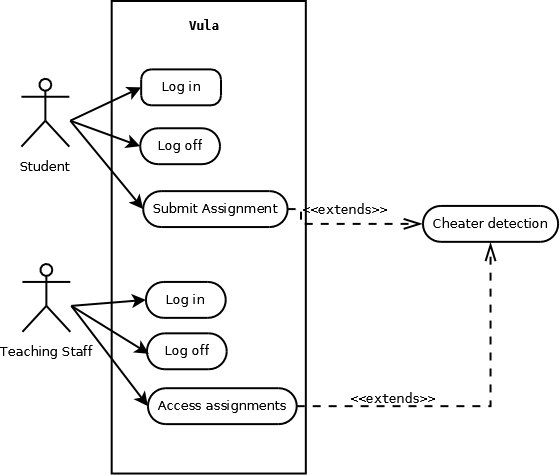
\includegraphics[scale=0.8]{use_case.png}}
  \caption{A use case diagram illustrating system interaction}
  \label{fig:usecase}
\end{figure}

\subsection{Functional Requirements}

\paragraph{Data integrity}
\begin{itemize}
    \item Data provided to the database must be correct, complete and coherent
    \item Data must be easily accessed whenever necessary
    \item Automated report generation with correct data
\end{itemize}

\paragraph{Information retrieval}
\begin{itemize}
    \item Retrieve matching pairs
    \item Retrieve list of marked cheated students
\end{itemize}

\paragraph{Authentication}
\begin{itemize}
    \item Must be accessible to UCT computer science students only
\end{itemize}

\paragraph{Database management}
\begin{itemize}
    \item General upkeep of database
    \item Store relevant data in a normalised format
\end{itemize}

\paragraph{Security}
\begin{itemize}
    \item Cheater checker data must be unavailable to students after they check their submissions.
    \item If security is breached, the software becomes redundant
\end{itemize}

\subsection{Non-functional Requirements}

\paragraph{Performance}
\begin{itemize}
    \item Cheater checker should be able to compute and check submissions within O(logN) 
\end{itemize}

\paragraph{Availability}
\begin{itemize}
    \item Must be available by lecturers even if Vula is down
\end{itemize}

\paragraph{Usability}
\begin{itemize}
    \item All users must be able to use the software easily because of an intuitive design
\end{itemize}

\paragraph{Capacity}
\begin{itemize}
    \item Must be able to handle the instance of all student submitting at once
\end{itemize}

\subsection{Usability Requirements}

\paragraph{Understandability}
\begin{itemize}
    \item Intuitive UI
    \item Easily understood results
    \item Easily identify Pairs of students with high likelihood of cheating from a list
    \item Easily identify Groups of students with high likelihood of cheating from a list
\end{itemize}

\paragraph{Learnability}
\begin{itemize}
    \item Complete documentation will be provided
    \item Explanation on how the system works for the designed context
    \item System relies on users recall rather than recognition
\end{itemize}

\paragraph{Operability}
\begin{itemize}
    \item Consistent UI elements
    \item Responsive UI interaction elements
    \item Reversible actions and constant feedback given 
    \item Responsive User interface design to accommodate varying screen resolutions
    \item Record students as having cheated individually from a Pair of students
    \item View list of students recorded for cheating to take action on them, instead of manually maintaining a spreadsheet.
\end{itemize}

\subsection{Artefacts produced}

A risk management assessment, relevant diagrams (such as class diagrams and architectural diagrams) and a gantt chart were produced in order to aid the development process in terms of time management and general direction. 

\begin{figure}[h!]
  \center{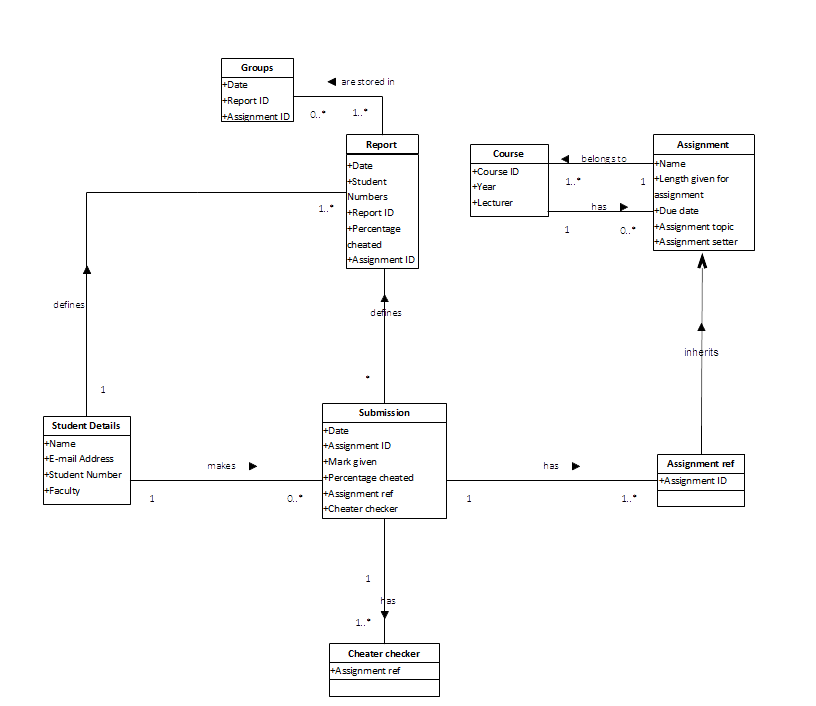
\includegraphics[scale=0.8]{analysis_class.png}}
  \caption{Analysis Class Diagram}
  \label{fig:analysisclass}
\end{figure}

\section{Design Overview}
\label{s:design-overview}

We have designed the system to be used from within an existing system (i.e. Vula) and it does not have to run as a standalone service. The system plugs into Vula to receive submissions. It then generates and stores signatures on the submission which get processed by a separate service that identifies matches and stores them. A lecturer reviews the results from the matching in the presentation layer and makes a decision as to whether the student should be marked for cheating or not. Submissions are categorised by their respective assignment, and are matched against submissions within that assignment over multiple years.

\paragraph{Algorithms used were}
\begin{itemize}
    \item The Winnower algorithm
    \item Grouper algorithm
    \item Suffix tree algorithm
\end{itemize}

\begin{figure}[h!]
  \center{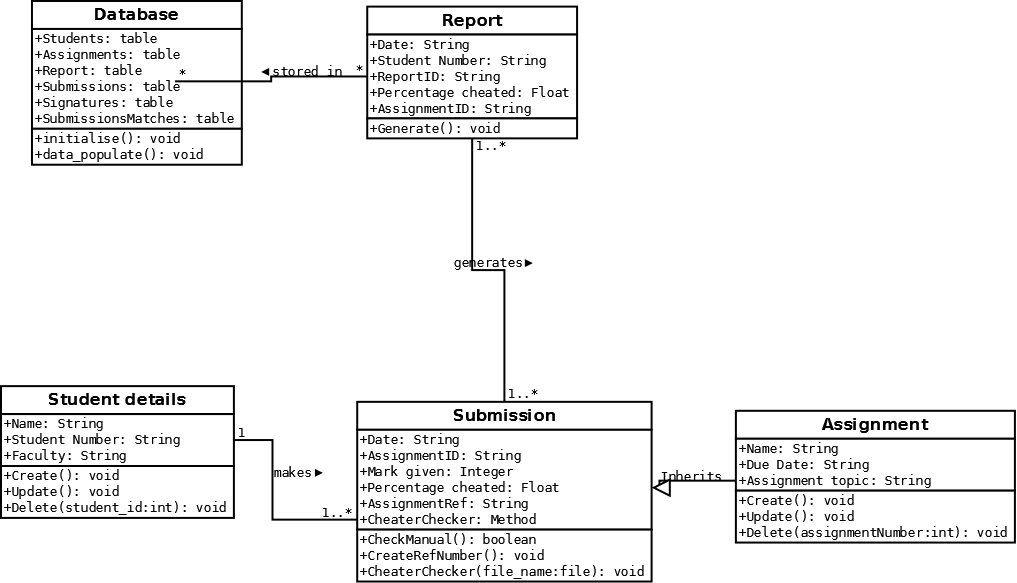
\includegraphics[scale=0.8]{design_class.png}}
  \caption{Design class diagram}
  \label{fig:designclass}
\end{figure}

\begin{figure}[h!]
  \center{\includegraphics[scale=0.8]{layerd_architecture.png}}
  \caption{Layered architectural diagram}
  \label{fig:layeredarchitecture}
\end{figure}



\section{Implementation}

\subsection{Data structures used}

\begin{figure}[h!]
  \center{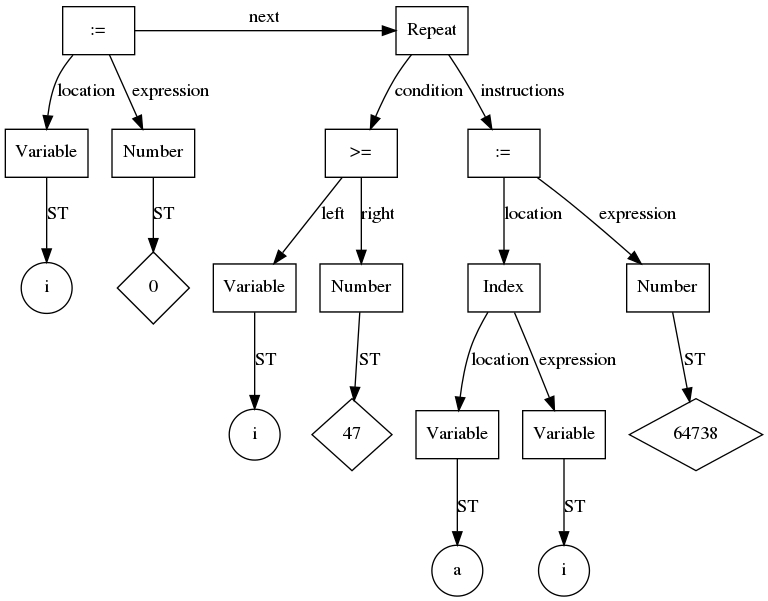
\includegraphics[scale=0.8]{abstract_syntax_tree.png}}
  \caption{Abstract Syntax Tree}
  \label{fig:abstractsyntaxtree}
\end{figure}

An Abstract syntax tree is generate a tree for programming syntax. The abstract syntax tree was used to generate signatures for comparison of submissions.

\begin{figure}[h!]
  \center{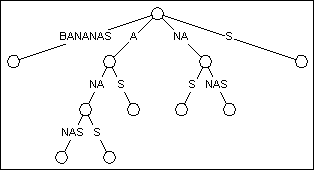
\includegraphics[scale=0.8]{suffix_tree.png}}
  \caption{Suffix Tree}
  \label{fig:suffixtree}
\end{figure}

The suffix tree is a tree structure which looks at the last part of a
given output. From the example, it gives all possible end combinations. This was
used to find the longest common substring in code.

\begin{figure}[h!]
  \center{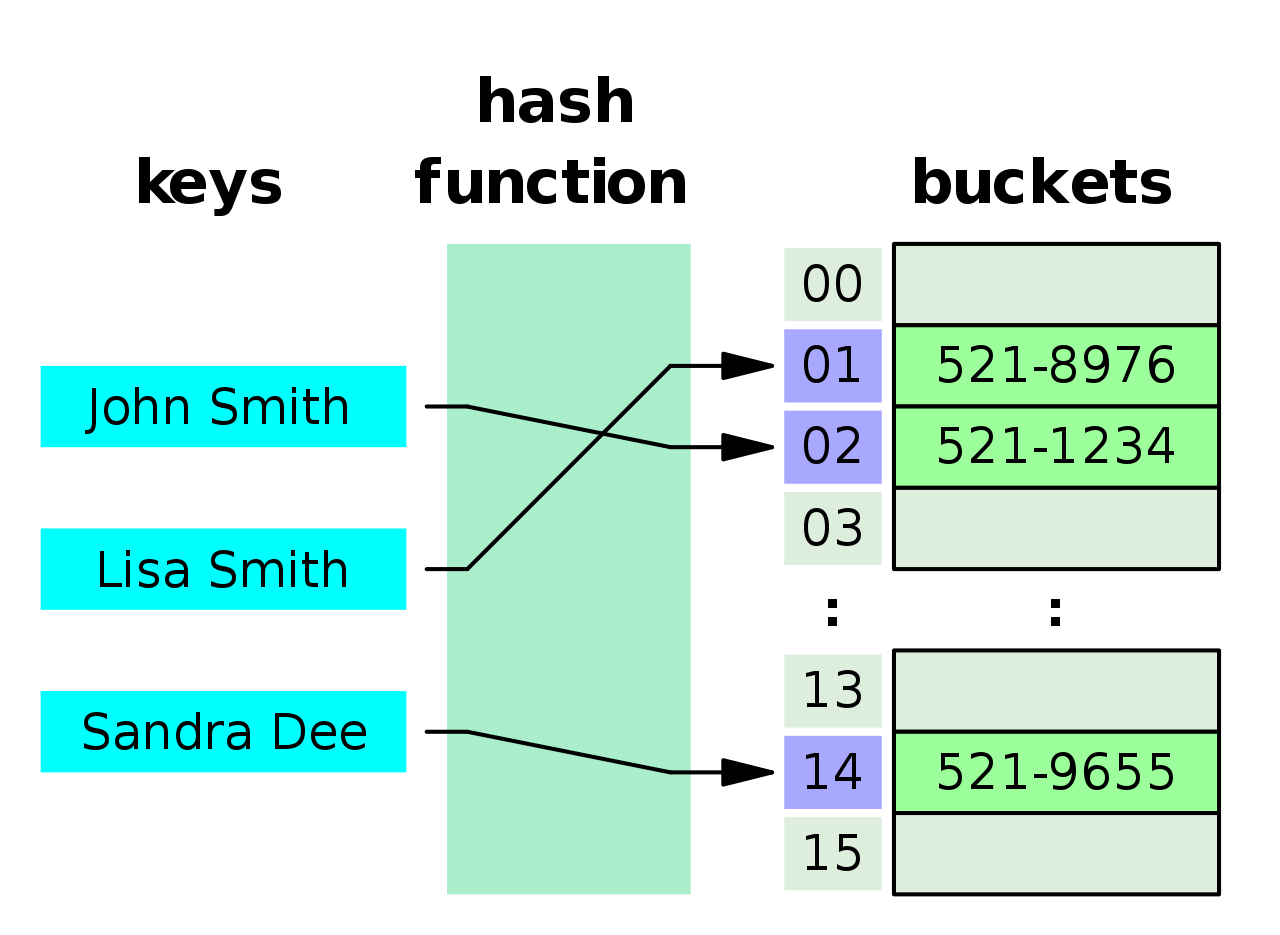
\includegraphics[scale=0.8]{hash_map.png}}
  \caption{Hash Map}
  \label{fig:hashmap}
\end{figure}

A hash map is used to implement an associative array. This means that  map keys to values. We used hashing to map between identifiers from once suspected instance of cheating to another for a greater measure of accuracy.


\section{User Interface features and implementation}

\begin{figure}[h!]
  \center{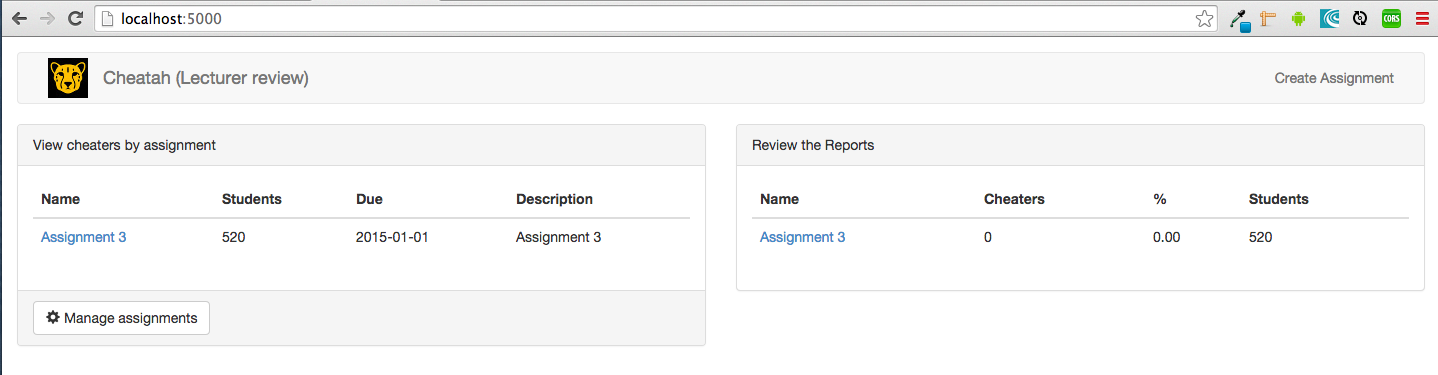
\includegraphics[scale=0.8]{ui_screenshot.png}}
  \caption{A screenshot of the UI on the home screen}
  \label{fig:uiscreenshot}
\end{figure}

The above image is an example of a screenshot from the home page. The UI was created using HTML and CSS for templating and Javascript for interaction. External libraries such as Bootstrap for CSS, D3.js for graphs, Prism.js for code highlighting, and jQuery were used. The implementation was done using the web framework called Flask.

\subsection{Overall design}

The user interface forms the front-end of the system which is served by the Flask server level and intended to be displayed in a modern browser. The interface was designed to be responsive in both its layout and functionality. It will adapt for optimal view on any reasonable screen resolution, and will also respond quickly to user interaction.  In order to achieve this some considerations needed to be taken into account, with their associated consequences. The biggest issue in supporting user interaction is cross browser compatibility. As this is not a functional requirement for the system, but a direct influence on the user’s ability to interact with it, it remains a critical concern. The following two paragraphs detail the solutions to this. 

The Bootstrap 3 CSS framework was used as a base level of CSS to enforce resets and layout rules that would make the UI responsive and compatible across browsers, backing up to Internet Explorer 8 and 9. On top of this, a style.css file was written to override Bootstrap’s CSS rules where necessary to accomplish the overall design. It was not necessary to make use of all of Bootstrap’s javascript libraries, so this is not included, but we make use of two of its smaller javascript files: alert.js so users can close alert dialogs; and dropdown.js for the dropdown menu in the navigation bar.

The considerations on cross browser javascript support in achieving responsive user interactions are less forgiving. Javascript runs single threaded in the browser and as a requirement needs to be non-blocking on the interface. In order to achieve a responsive and non-blocking interface the UI needs to make any combination of HTTP requests to the Flask server layer in an asynchronous manner. Such asynchronous requests are generally written with function calls that get given, as parameters, callback functions. These callback functions are to be executed on receiving a response from the server, and get passed either an error or the result from the server’s response. This leads to heavily nested, unmaintainable code which is hard to read. As a result, a design decision in favour of maintainability and readability was made for asynchronous requests to have to be made by a concept called Promises. Promises allow for chaining of asynchronous request/response calls. The code is more intuitive to read and avoids nesting, however it is limited to modern browsers from Firefox version 30, Chrome version 33, Opera version 23, and Safari version 8 and up. A polyfill can be included, providing support for Promises in browsers dating back to Internet Explorer 9, but this was not included due to time constraints and the assumption that users of the system would be from the Computer Science department, which is a controlled environment that likely runs up to date browsers.

\subsection{Dynamic pages and dynamic interaction}

The considerations on cross browser javascript support in achieving responsive user interactions are less forgiving. Javascript runs single threaded in the browser and as a requirement needs to be non-blocking on the interface. In order to achieve a responsive and non-blocking interface the UI needs to make any combination of HTTP requests to the Flask server layer in an asynchronous manner. Such asynchronous requests are generally written with function calls that get given, as parameters, callback functions. These callback functions are to be executed on receiving a response from the server, and get passed either an error or the result from the server’s response. This leads to heavily nested, unmaintainable code which is hard to read. As a result, a design decision in favour of maintainability and readability was made for asynchronous requests to have to be made by a concept called Promises. Promises allow for chaining of asynchronous request/response calls. The code is more intuitive to read and avoids nesting, however it is limited to modern browsers from Firefox version 30, Chrome version 33, Opera version 23, and Safari version 8 and up. A polyfill can be included, providing support for Promises in browsers dating back to Internet Explorer 9, but this was not included due to time constraints and the assumption that users of the system would be from the Computer Science department, which is a controlled environment that likely runs up to date browsers.

The Flask server layer makes use of a templating engine called jinja which is used to render dynamic web pages from templates. These web pages are dynamic from the context of the server in that data is injected into the template to render the page. This data is variable and often depends on results from database queries. From the users perspective, however, these are static pages which do not respond to interaction other than to perform a full page refresh or navigate to another URL. In some circumstances this is grossly inefficient for interaction and in these situations javascript is used to enhance functionality on the page, providing dynamic user interaction which is highly responsive and time efficient.

Once again browser compatibility is a concern as different browsers can have inconsistencies with their javascript implementations. In order to meet this shortfall, many checks have to be performed on the type of browser, which then run different implementations of the same javascript code. This is unmaintainable and as a result jQuery was used, which serves to abstract away these differences while also allowing for shorter, cleaner javascript code. jQuery version 2.1 was used, which is supported by Internet Explorer 9 and above.

Fortunately not all views require dynamic user interaction and as a result the
crux of the javascript code base is isolated to just one view, the cheaters\_review.html page, where lecturers review code from student submissions marked for plagiarism and then decide to record students as having cheated or not. The following paragraph details the view and the javascript implementation to achieve the interaction, all remaining views do not need dynamic javascript interaction and perform relatively straight forward CRUD (Create, Read, Update and Delete) operations on the database.

\subsection{Dynamic interaction for reviewing cheaters}

The purpose of the cheaters\_review.html view is to display instances of possible cheating. Such an instance is a pair of submissions which are similar to one another, and as a result the data we work with is a list of pairs of students each with their notably similar submission. The students in a pair are each rated by the number of common lines, as well as a percentage based on this number to the total number of lines in their submission.

This list of pairs tends to be long, and the lecturer needs to be able to intuit the degree of plagiarism by the ratings which are provided. It was detailed in a client review meeting that the use case for this is by observing the rating of the top few listings and tracing down the list for as long as the level remains more or less consistent. When the level falls off drastically it can be assumed that the likelihood of cheating for the remaining students does so as well. To aid  in determining where this threshold lies a histogram is displayed, to the right of the list of pairs, illustrating the number of students in the different percentage ranges.

\begin{figure}[h!]
  \center{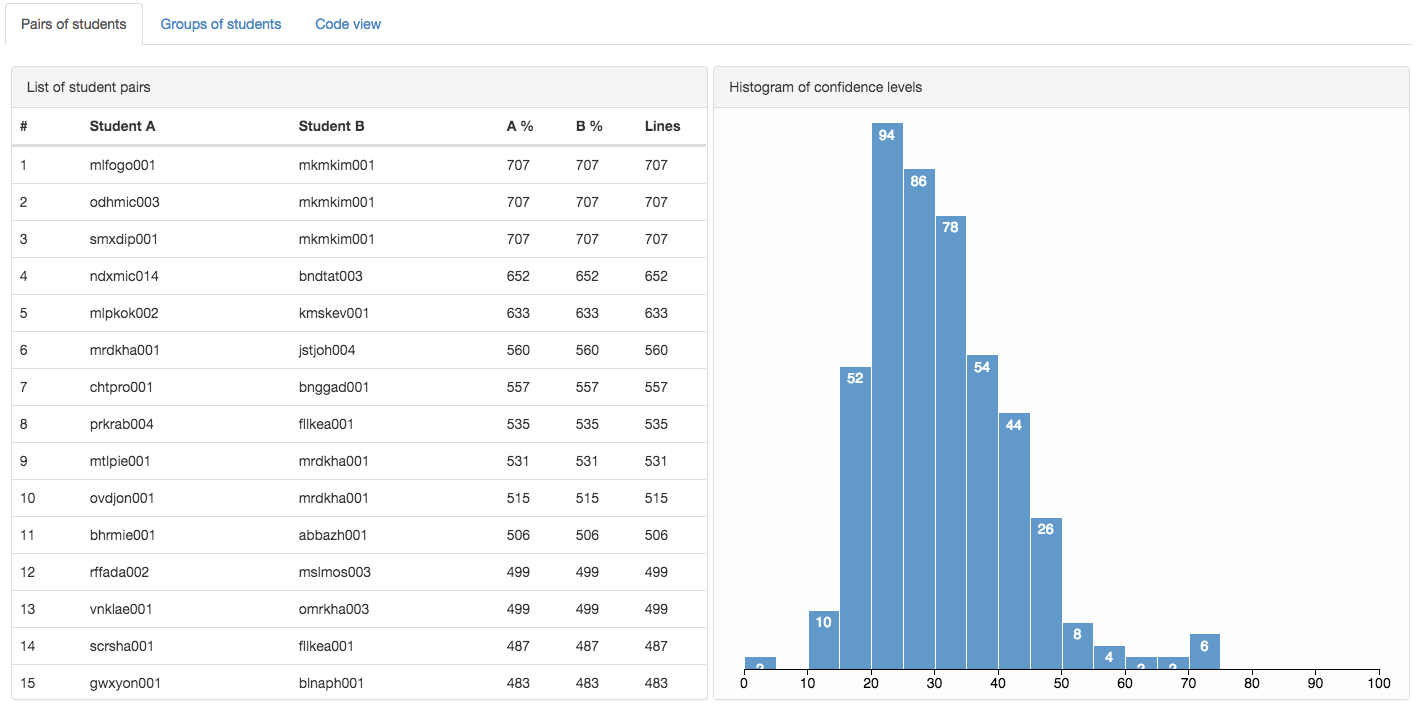
\includegraphics[scale=0.8]{pairs_histogram.png}}
  \caption{A screenshot of the pairs of students and the corresponding histogram}
  \label{fig:pairshistogram}
\end{figure}

When a lecturer wants to compare code they just have to click on a list pair and the view will switch its focus to a code view displaying the code of the two students side by side. The exact line numbers which match are fetched asynchronously and displayed clearly in highlighted blocks over the code. Above the code blocks there is an action bar which contains dynamically rendered buttons containing the common line numbers, and will scroll the code to the respective line number when clicked.

\begin{figure}[h!]
  \center{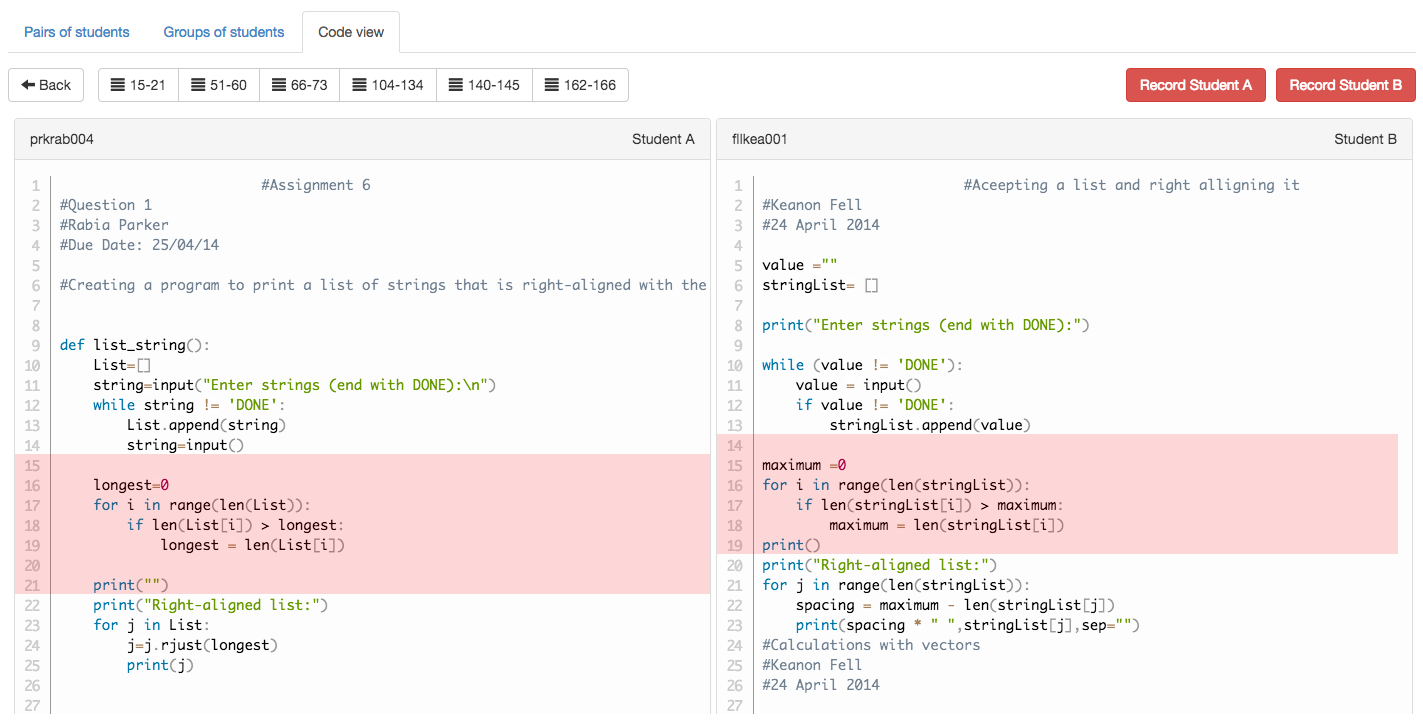
\includegraphics[scale=0.8]{code_view.png}}
  \caption{A screenshot of the copied regions of code}
  \label{fig:codeview}
\end{figure}

Horizontal and vertical scrolling in the left code block is mirrored by the right code block. This is a design decision made due to the fact that line numbers do not match up one-to-one and are sometimes offset by a fair amount. It is also a result of a limitation with the javascript plugin used for the code highlighting. The design decision is a compromise which allows the user to reach highlighted lines of code in the left block, and then scroll independently in the right code block to make up the offset and view the lines side by side. If scrolling was mirrored in a bidirectional fashion it would be somewhat impractical.

Two buttons exist in the action bar for recording either student independently as having cheated. This is necessary for the use case where the lecturer determines that only one student has cheated. The buttons trigger an asynchronous request to record the respective student as a cheater for the given assignment. The text in the buttons responds accordingly and reflects the state of the request. For example, the button text could read “Record Student A”, upon click that will change to “Recording…” and on successful completion will change to “Undo”. “Undo” means that the transaction has been successful, and it can be reverted if this was made unintentionally by human error. Pressing the button while in the “Undo” state will send an asynchronous delete request and revert the system back to it’s original state. This serves our operability requirement in providing reversible actions and constant feedback.

A back button is provided in the action bar to conveniently return back to the previous listing and continue after the lecturer has finished reviewing the code.

\subsection{Listing students in Groups}

It is often the case that code is shared among a group of students, not just two. The listing of student pairs is linear and provides no information as to the relationship among student pairs. It is useful for the lecturer, and a requirement of the system, to be able to see the extent of cheating by knowing about these groups of students with similar code. To meet this requirement we have an additional listing containing Groups of student pairs. This listing is built upon the data containing the student pairs and feeds the pair into a graph with the students as nodes and the pair as an edge connecting them. The graph is then traversed and it identifies groups by isolated clusters of students. These groups are then listed with the pairs that make up the group, containing the same information as on the Pairs listing but just categorised by group. Clicking on a pair in a group will render the graph representing the entire group into the diagram on the right of the group listing. This graph gives a visual illustration of how the group is related and a star shaped graph quickly identifies the student most likely to have shared the code. Clicking on an edge in the graph will select the pair and focus the view onto their code in precisely the same way as in the Pairs listing.

\begin{figure}[h!]
  \center{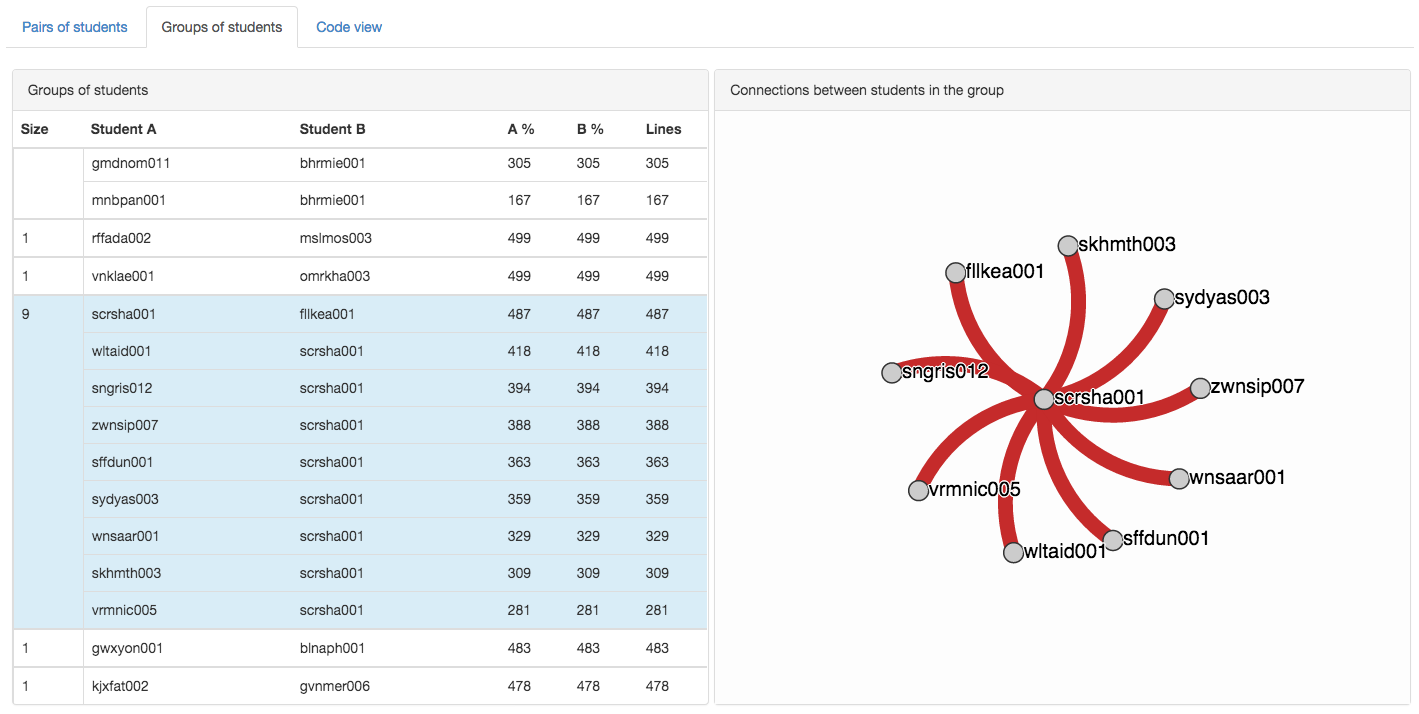
\includegraphics[scale=0.8]{group_view.png}}
  \caption{A screenshot of the group view with a star topology graph}
  \label{fig:graphview}
\end{figure}

\subsection{Reports on cheating students}

A use case for acting on instances of cheating is to manually copy the offending student numbers over into an excel spreadsheet. This spreadsheet is then referenced when assigning students zero or taking further action on them. The system meets this use case by providing a report page which lists the students that have been marked for cheating by assignment. A button is provided on the report pages which will download the list as a CSV file in the case where a lecturer needs to use the data elsewhere. The downloaded CSV file is named according to the assignment number for easy identification. A button also exists to delete students from the listing. This is either in the case where a student has been added in error, or the student has been resolved or assigned zero and no longer needs to be listed.

\begin{figure}[h!]
  \center{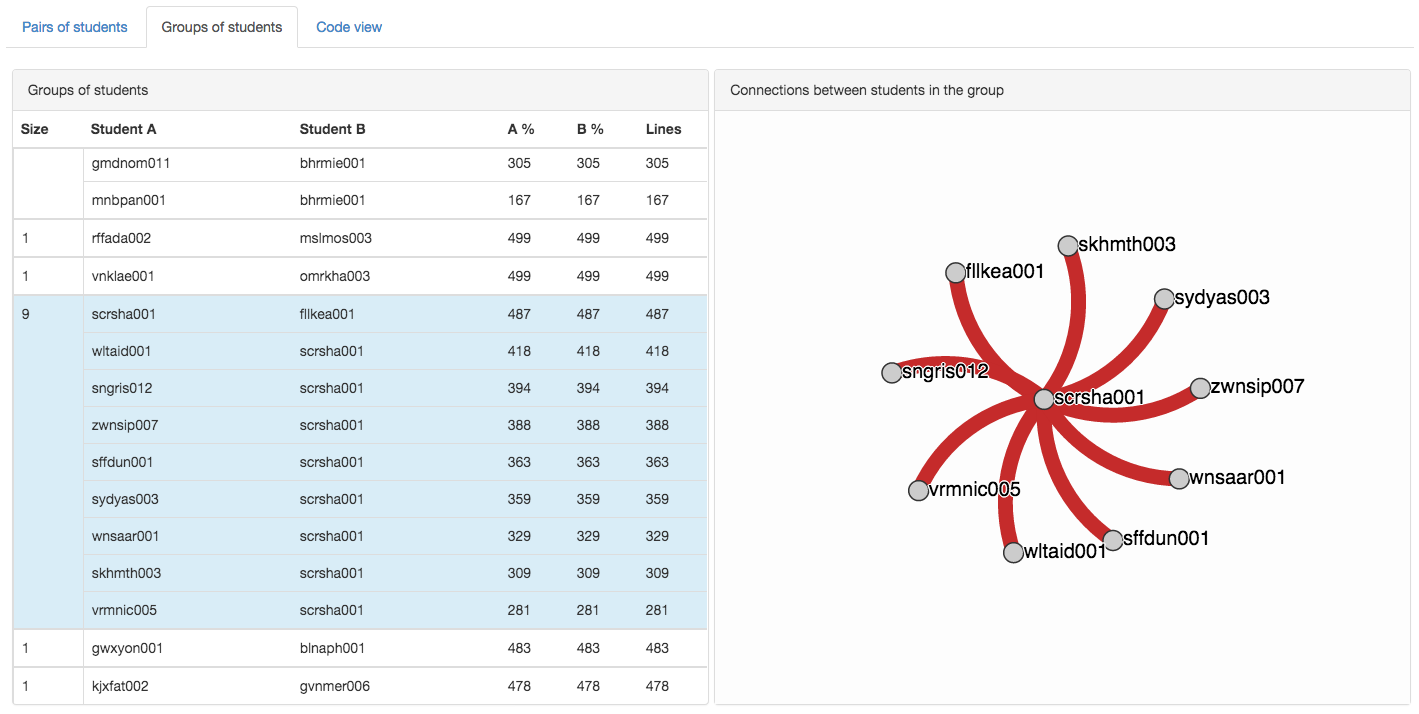
\includegraphics[scale=0.8]{group_view.png}}
  \caption{A screenshot of the report view, listing students that have been
  marked as cheating on an assignment}
  \label{fig:graphview}
\end{figure}


\section{General overview of the entire system}

\begin{figure}[h!]
  \center{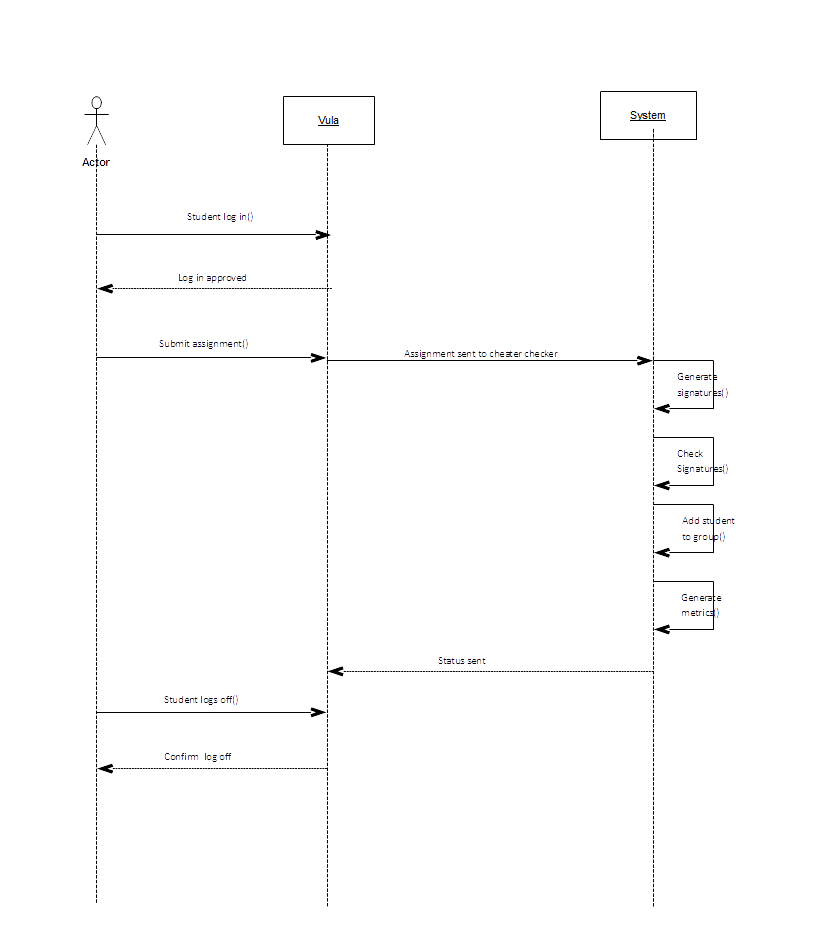
\includegraphics[scale=0.8]{sequence_diagram.png}}
  \caption{A sequence diagram to indicate how the system works}
  \label{fig:sequencediagram}
\end{figure}

\paragraph{All classes are grouped into groups based on their use. The groups of
classes are}
\begin{itemize}
\item Algorithms
\item Database
\item External
\item Languages
\item Model
\item Scraper
\item Tests 
\item UI
\end{itemize}

Selecting the most important method in each class will be close to impossible as each method is needed. Code has been stripped of redundant methods so every method in each class is equally important.

\subsection{Relationship between classes}

\textit{BaseAlgorithm abstract class}
Abstract class for detection algorithm which defines methods.

\textit{WinnowingAlgorithm extends BaseAlgorithm}
Implements a string matching algorithm (similar to the one implemented by the MOSS
system) for signature generation and signature matching.

\textit{Program}
Represents a submission by the user and stores our cheating detections

\textit{PythonProgram extends Program}
Implements Python specific parsing to remove variable and function names

\subsection{Special programming techniques}

Test driven development was used to make code more efficient and reduce occurrences of errors in the code. Automated testing was used for this same reason, to catch bugs as they occurred.

\subsection{Libraries}

Libraries plyj and  ply were used to parse code from submission to the system to be evaluated. Sqlite3 was used for database management. Flask was used as a web framework for the presentation layer of the system and to make calls to the database manager.


\section{Program Validation and Verification}
\label{ss:progr-valid-verif}

Tell us how you tested the system and why you believe it works.
Describe all the steps taken to validate the correctness of the
program.

If you had user tests then say what you did and what the results
were. Describe why these test data were chosen (what test conditions
the data was testing).  Table \ref{tab:tests} provides an example of
the sorts of results we are looking for. The full detail of the test
runs should be appended to the report.

\begin{table}[h!]
  \centering
\caption{A table of tests. A table caption goes above the table.}

  \begin{tabular}[t]{|p{5cm}|p{3cm}|p{3cm}|p{3cm}|} 
      \hline 
          \textbf{Data Set and reason for its choice} & 
          \multicolumn{3}{c|}{\textbf{Test Cases}}
          \\
          \cline{2-4} & 
            \emph{Normal Functioning} & 
            \emph{Extreme boundary cases} &
            \emph{Invalid Data (program should not crash)} 
          \\ 
          \hline 
            Syntax error in submission file & 
            Passed & 
            Syntax errors & 
            Ignored
          \\
          \hline 
            Database management testing &
            Passed &
            Invalid inputs were ignored &
            Removed to ensure normalisation
          \\ 
          \hline
            Detection algorithm testing &
            Passed &
            &
          \\ 
          \hline
            Flask server testing &
            Passed &
            n/a &
            None
          \\
          \hline
              Testing the suffix tree &
              Passed &
              &
          \\
          \hline
            Testing the suffix tree algorithm &
            Passed &
            Long files were passed to the algorithm. &
            None
          \\
          \hline
            Testing the winnower algorithm &
            Passed &
            None &
            None
          \\
          \hline
            Test the canonicalisation &
            Passed &
            None &
            None
          \\
          \hline
          Test the Runner &
          Passed &
          &
          \\
          \hline
  \end{tabular}

\label{tab:tests}
\end{table}

Follow your table of results with a discussions of them highlighting
how useful and usable your system is for its intended purpose.

\section{Conclusion}
\label{ss:conclusion}

Your report must have a clear conclusion where you revisit the aims
set out in the beginning and discuss how well you met them. Did you
achieve the objective of creating a well-structured, modular, and
robust system?  Please summarize the design features and test results
that show this.

\begin{thebibliography}{9}

\bibitem[Kopka and Daly(2004)]{KopkaDaly}
Kopka, H. and Daly, P.W.  (2004) \textit{A Guide to \LaTeXe:
Document Preparation for Beginners and Advanced Users} (4th~edn).
Addison-Wesley.

\bibitem[Lamport(1994)]{Lamport}
Lamport L. (1994) \textit{\LaTeX: A Document Preparation System}
(2nd~edn). Addison-Wesley.

\bibitem[Mittelbach and Goossens(2004)]{Companion}
Mittelbach, F. and Goossens, M., (2004) \textit{The \LaTeX\
Companion} (2nd~edn). Addison-Wesley.

\end{thebibliography}
\end{document}
